\documentclass[11pt,a4paper]{article}

% ---------------------------------------------------------------- packages
\usepackage[utf8]{inputenc}
\IfFileExists{lmodern.sty}{\usepackage[T1]{fontenc}\usepackage{lmodern}}{}
\usepackage[english]{babel}
\usepackage[a4paper,margin=2.5cm]{geometry}
\usepackage{microtype}
\usepackage{amsmath,amssymb}
\usepackage{graphicx}
\usepackage{booktabs}
\usepackage[font=small,labelfont=bf,skip=6pt]{caption}
\usepackage[round,authoryear]{natbib}
\usepackage{xcolor}
\definecolor{linkblue}{HTML}{1F5FAD}
\definecolor{dagnode}{HTML}{E9E8E4}
\definecolor{dagrating}{HTML}{EB6834}
\definecolor{dagsent}{HTML}{2A78D6}
\definecolor{boxbg}{HTML}{F6F5F2}
\usepackage[colorlinks=true,linkcolor=linkblue,citecolor=linkblue,urlcolor=linkblue]{hyperref}
\usepackage{titlesec}
\titleformat{\section}{\large\bfseries}{\thesection}{0.6em}{}
\titleformat{\subsection}{\normalsize\bfseries}{\thesubsection}{0.6em}{}
\titlespacing*{\section}{0pt}{14pt}{6pt}
\titlespacing*{\subsection}{0pt}{10pt}{4pt}
\setlength{\parskip}{3pt}
\usepackage{enumitem}
\usepackage{tikz}
\usetikzlibrary{arrows.meta}
\usepackage{fvextra}

\newcommand{\pred}[1]{\textbf{P#1}}

% ---------------------------------------------------------------- title
\title{\vspace{-1.2cm}\textbf{Is Good Food Really Enough to Get\\ 5 Stars on Google Maps?}\\[4pt]
\large What Drives Customer Satisfaction in Parisian Restaurants}
\author{Nathan Tessot\\[2pt]
\small CPES -- Data Science \& Cultural Sciences, Université PSL\\
\small Applied data science project}
\date{\small April 2026}

\begin{document}
\maketitle

% ---------------------------------------------------------------- abstract
\begin{abstract}
\noindent
This paper examines the key drivers of customer satisfaction in the Parisian
restaurant industry by analyzing Google Maps reviews. Using a large language
model to extract granular scores on six dimensions (food quality, value for
money, service, wait time, atmosphere and cleanliness) from 5,000 reviews, we
estimate their respective association with the star rating and with the
overall sentiment of each review. Food quality is by far the most important
factor ($\beta = 0.54$ for the rating), followed by service quality
($\beta = 0.26$).
Value for money and atmosphere also play significant roles, while wait time
and cleanliness have a smaller, though still positive, effect. The
restaurant's popularity has no detectable influence. These findings suggest
that while a holistic experience matters, culinary excellence and attentive
service remain the primary pillars of restaurant success in competitive urban
markets.
\end{abstract}

% ---------------------------------------------------------------- 1
\section{Introduction}

Reputation on Google Maps has become a major concern for restaurant owners
since the platform became a standard way of finding places to eat
\citep{li2020}. More generally, in the digital economy, online reviews shape an
establishment's reputation and have a measurable impact on revenue
\citep{luca2016}. Beyond the digital context, understanding customer reviews
also requires the broader theory of consumer perception, which holds that the
perceived value of an experience is a trade-off between price, quality and
personal benefit \citep{zeithaml1988}.

Google reviews are a particularly interesting case because ratings form the
digital identity of an establishment. While exceptional food is traditionally
the main reason people go to a restaurant, a dining experience is shaped by
many other factors: a friendly waiter, a pleasant atmosphere or the perceived
value for money can strongly influence how a customer feels. This study
therefore investigates how these elements relate to the score a customer
decides to leave, and to the overall positive or negative sentiment of the
review.

\begin{center}
\emph{Which aspects of a dining experience are most strongly associated with a
good rating and a positive sentiment on Google Maps?}
\end{center}

Figure~\ref{fig:dag} summarizes the hypothesized relationships. Based on
them, we formulate four predictions:

\begin{enumerate}[label=\pred{\arabic*}, leftmargin=2.2em, itemsep=1pt]
  \item Food quality is the strongest predictor of a high rating,
  significantly outweighing the other factors.
  \item People tend to give higher ratings to restaurants that are already
  popular and have a large number of reviews.
  \item Since human interactions still matter, service quality is a strong
  factor explaining a positive sentiment.
  \item The restaurant setting, such as its atmosphere and cleanliness, is a
  strong predictor of a positive sentiment.
\end{enumerate}

\begin{figure}[t]
\centering
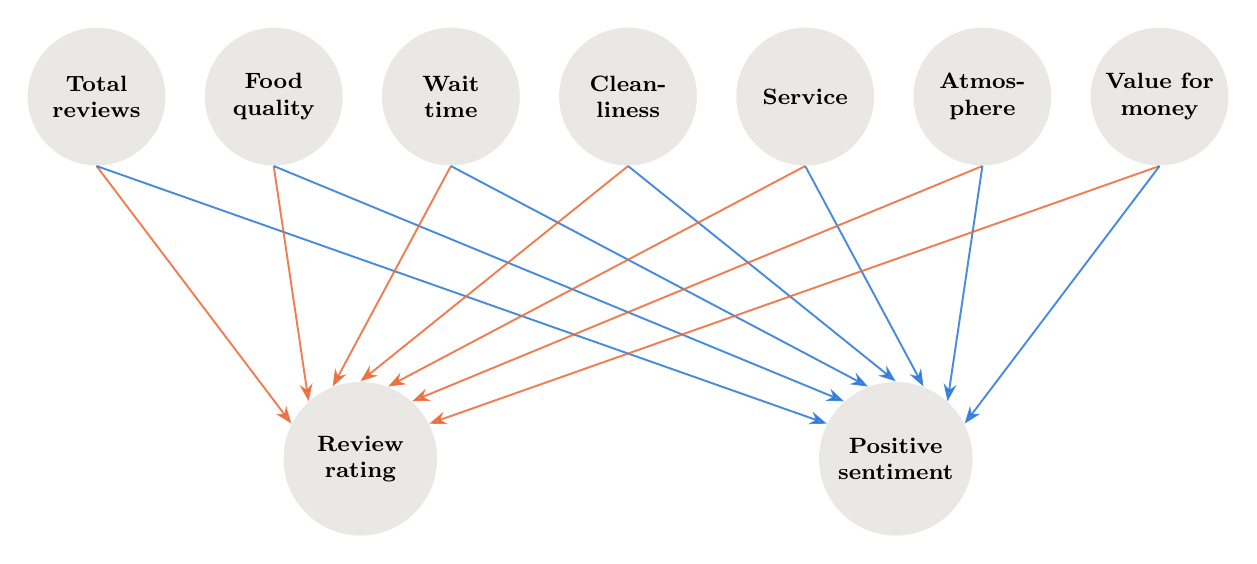
\begin{tikzpicture}[
  x=1cm, y=1cm,
  var/.style={circle, fill=dagnode, minimum size=1.75cm, inner sep=0pt,
              align=center, font=\footnotesize\bfseries},
  outv/.style={circle, fill=dagnode, minimum size=1.95cm, inner sep=0pt,
              align=center, font=\footnotesize\bfseries},
  ar/.style={-{Stealth[length=2.2mm]}, line width=0.7pt, opacity=0.85},
]
  \foreach \name/\lab [count=\i] in {tr/Total\\reviews, fq/Food\\quality,
      wt/Wait\\time, cl/Clean-\\liness, sv/Service, at/Atmos-\\phere,
      vm/Value for\\money}
    \node[var] (\name) at ({(\i-4)*2.25}, 0) {\lab};
  \node[outv] (rr) at (-3.4,-4.6) {Review\\rating};
  \node[outv] (ps) at ( 3.4,-4.6) {Positive\\sentiment};
  \foreach \name [count=\i] in {tr,fq,wt,cl,sv,at,vm} {
    \pgfmathsetmacro{\ang}{153-21*(\i-1)}
    \draw[ar, dagrating] (\name.south) -- (rr.\ang);
    \draw[ar, dagsent]   (\name.south) -- (ps.\ang);
  }
\end{tikzpicture}
\caption{Hypothesized relationships (DAG). Orange arrows point to the review
rating, blue arrows to the positive sentiment. Relationships between the
criteria themselves are not shown, for readability.}
\label{fig:dag}
\end{figure}

% ---------------------------------------------------------------- 2
\section{Data}

The dataset was collected in March 2026. Using the Google Maps Places API, we
first retrieved the identifier of each Parisian restaurant, along with its
address, the number of user reviews it has received and the text of these
reviews.

We then drew a representative sample of Parisian restaurants, selecting the
same proportion of restaurants at each rating level as in the API results.
The final dataset contains $N = 5{,}000$ reviews from about 3{,}800
restaurants (Figure~\ref{fig:desc}). Each review was annotated
by the Qwen2.5 language model, which assigned a score from $-2$ (very negative)
to $+2$ (very positive), with $0$ meaning neutral or not mentioned, for six
criteria: \textbf{food quality}, \textbf{value for money}, \textbf{service},
\textbf{wait time}, \textbf{atmosphere} and \textbf{cleanliness}. The model
also assigned a binary sentiment score (1 if the review is generally positive,
0 otherwise). To improve reliability, it was asked to justify its scores in
one sentence and to score 0 any criterion not explicitly mentioned; the full
prompt is given in Appendix~\ref{app:prompt}.

Each review is thus described by seven features: the six criteria above, plus
the total number of reviews of the restaurant, used as a measure of its
popularity.

\begin{figure}[t]
  \centering
  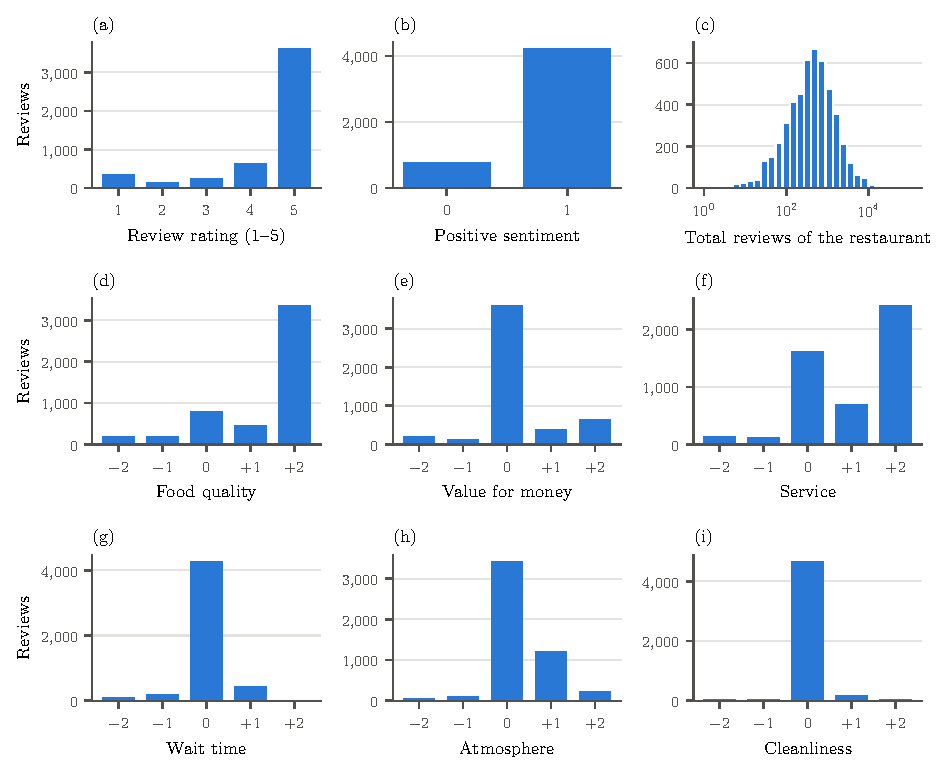
\includegraphics[width=\linewidth]{figures/fig2_descriptives.pdf}
  \caption{Univariate description of the dataset: (a)~review rating,
  (b)~positive sentiment, (c)~total number of reviews of the restaurant
  (log scale), (d)~food quality, (e)~value for money, (f)~service,
  (g)~wait time, (h)~atmosphere, (i)~cleanliness. Criteria are scored from
  $-2$ to $+2$, with $0$ when not mentioned.}
  \label{fig:desc}
\end{figure}

% ---------------------------------------------------------------- 3
\section{Method}

To test the predictions, we estimate two multiple linear regressions (OLS),
explaining respectively the star rating given by the user and the overall
sentiment of the review. All variables, outcomes included, are standardized
beforehand, so each coefficient $\beta$ is the change in the outcome, in
standard deviations, associated with a one-standard-deviation increase in the
predictor. This makes the effects of the different criteria directly
comparable.
\begin{align}
\text{Rating}_i &= \beta_0 + \beta_1\,\text{Food}_i + \beta_2\,\text{Value}_i
  + \beta_3\,\text{Service}_i + \beta_4\,\text{Wait}_i
  + \beta_5\,\text{Atmosphere}_i \nonumber\\
  &\quad + \beta_6\,\text{Cleanliness}_i + \beta_7\,\text{TotalReviews}_i
  + \varepsilon_i \\[4pt]
\text{Positive}_i &= \beta_0 + \beta_1\,\text{Food}_i + \beta_2\,\text{Value}_i
  + \beta_3\,\text{Service}_i + \beta_4\,\text{Wait}_i
  + \beta_5\,\text{Atmosphere}_i \nonumber\\
  &\quad + \beta_6\,\text{Cleanliness}_i + \beta_7\,\text{TotalReviews}_i
  + \varepsilon_i
\end{align}

% ---------------------------------------------------------------- 4
\section{Results}

Table~\ref{tab:results} and Figure~\ref{fig:forest} summarize both models.

\begin{table}[h]
  \centering
  \small
  \begin{tabular}{lrrrr}
    \toprule
    & \multicolumn{2}{c}{(1) Review rating} & \multicolumn{2}{c}{(2) Positive sentiment} \\
    \cmidrule(lr){2-3}\cmidrule(lr){4-5}
    Predictor & $\beta$ & $p$ & $\beta$ & $p$ \\
    \midrule
    Food quality      & 0.538 & $<0.001$ & 0.566 & $<0.001$ \\
    Service           & 0.261 & $<0.001$ & 0.231 & $<0.001$ \\
    Value for money   & 0.156 & $<0.001$ & 0.127 & $<0.001$ \\
    Atmosphere        & 0.097 & $<0.001$ & 0.093 & $<0.001$ \\
    Wait time         & 0.047 & $<0.001$ & 0.058 & $<0.001$ \\
    Cleanliness       & 0.041 & $<0.001$ & 0.007 & 0.442 \\
    Total reviews     & 0.011 & 0.227    & $-0.010$ & 0.287 \\
    \midrule
    $R^2$             & \multicolumn{2}{c}{0.60} & \multicolumn{2}{c}{0.58} \\
    \bottomrule
  \end{tabular}
  \caption{Standardized coefficients of the two multiple regressions
  ($N = 5{,}000$ reviews, OLS).}
  \label{tab:results}
\end{table}

\begin{figure}[h]
  \centering
  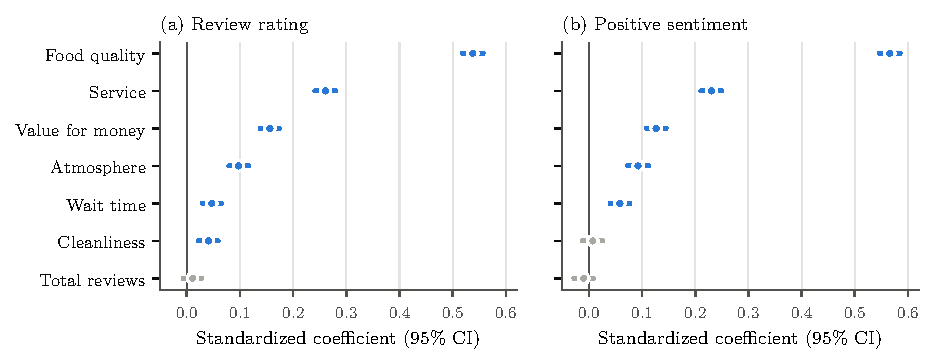
\includegraphics[width=\linewidth]{figures/fig3_forest.pdf}
  \caption{Standardized coefficients with 95\% confidence intervals:
  (a)~review rating, (b)~positive sentiment. Grey marks a non-significant
  effect.}
  \label{fig:forest}
\end{figure}

\subsection{Review rating}

The first model explains a large share of the variance ($R^2 = 0.60$). As
expected, food quality is the primary driver of the numerical rating
($\beta = 0.54$, $p < 0.001$; Figure~\ref{fig:forest}a), which strongly supports
\pred{1}: its coefficient is about twice that of any other criterion.

Beyond culinary attributes, the results confirm the importance of the human
and physical dimensions of the dining experience. Service quality is the
second most influential factor ($\beta = 0.26$, $p < 0.001$). Value for money
($\beta = 0.16$), atmosphere ($\beta = 0.10$), wait time ($\beta = 0.05$) and cleanliness
($\beta = 0.04$) are all positively and significantly associated with the star
rating ($p < 0.001$).

\pred{2}, the ``popularity effect'', is not supported: the total number of
reviews has no significant effect on individual ratings ($p = 0.227$). This
suggests that customers tend to evaluate their experience on its own terms,
regardless of the restaurant's existing reputation.

\subsection{Positive sentiment}

The second model ($R^2 = 0.58$) yields structurally similar results. Food
quality ($\beta = 0.57$, $p < 0.001$; Figure~\ref{fig:forest}b) and service
($\beta = 0.23$, $p < 0.001$) remain by far the dominant variables, which supports
\pred{3}: service quality has a substantial association with a positive
review. Value for money ($\beta = 0.13$), atmosphere ($\beta = 0.09$) and wait time
($\beta = 0.06$) remain significant ($p < 0.001$), while the restaurant's
popularity again has no effect ($p = 0.287$).

The main difference between the two models concerns cleanliness. While it
slightly influences the numerical rating, it is not significantly associated
with an overall positive sentiment ($p = 0.442$). \pred{4} is therefore only
partly supported: the physical setting matters, mostly through atmosphere,
but cleanliness alone is not enough to secure a positive review. This may
partly reflect how rarely cleanliness is mentioned at all
(Figure~\ref{fig:desc}i).

% ---------------------------------------------------------------- 5
\section{Conclusion}

Customer satisfaction on Google Maps follows a clear hierarchy: food quality
and service substantially outweigh value for money, atmosphere, wait time and
cleanliness. While a holistic approach to service and setting is valuable,
excelling in food quality and in the human side of service remains the most
direct path to high ratings. Moreover, the absence of any association between
a restaurant's review volume and its individual scores suggests that users
judge their own experience rather than follow the crowd.

These results come with limitations. The scores are produced by a language
model, whose annotations may contain errors; most criteria are absent from
most reviews, which limits the precision of their estimates; some
restaurants contribute several reviews, so observations are not fully
independent; and the regressions describe associations, not causal
effects.

They also open new questions about the socio-geographical context. A
promising next step would be to test whether these satisfaction drivers
differ between tourist-heavy and residential districts of Paris. Exploring how
location and local competition moderate these relationships would give a more
nuanced understanding of urban consumer behavior in the digital age.

% ---------------------------------------------------------------- refs
\begin{thebibliography}{99}
\setlength{\itemsep}{1pt}\small

\bibitem[Li and Hecht(2020)]{li2020}
Li, Z., \& Hecht, B. (2020). 3 stars on Yelp, 4 stars on Google Maps: A
cross-platform examination of restaurant ratings. \emph{Proceedings of the
ACM on Human-Computer Interaction}, 4(CSCW2), 1--24.

\bibitem[Luca(2016)]{luca2016}
Luca, M. (2016). Reviews, reputation, and revenue: The case of Yelp.com.
\emph{Harvard Business School Working Paper}, No.~12-016.

\bibitem[Zeithaml(1988)]{zeithaml1988}
Zeithaml, V.~A. (1988). Consumer perceptions of price, quality, and value: A
means-end model and synthesis of evidence. \emph{Journal of Marketing},
52(3), 2--22.

\end{thebibliography}

% ---------------------------------------------------------------- appendix
\appendix
\section{Annotation prompt}
\label{app:prompt}

System prompt sent to the language model for review annotation (written in
French).

\VerbatimInput[fontsize=\scriptsize, breaklines=true, breaksymbolleft={},
  frame=single, rulecolor=\color{dagnode}, framesep=3mm,
  formatcom=\color{black!85}]{prompt.txt}

\end{document}
